\documentclass[12pt]{book}

\usepackage{natbib} % Tidies up citation numbers.
\usepackage[utf8]{inputenc}
\usepackage{graphicx}
\usepackage{pythonhighlight}
\usepackage{listingsutf8}
\usepackage{float}

%\def\UrlBreaks{\do\/\do-}
\usepackage[T1]{fontenc}
\usepackage{url}
\usepackage{breakurl}

\usepackage{pdfpages}

\lstset{
  extendedchars=true,
  language=java,
  basicstyle=\tiny\ttfamily,
  showspaces=false,
  showstringspaces=false,
    literate=
     {É}{{\'E}}{1}%
      {Á}{{\'A}}{1}%
      {Ã}{{\~A}}{1}%
      {Â}{{\^A}}{1}%
      {À}{{\`A}}{1}%
      {Ç}{{\,C}}{1}%
      {Ó}{{\'O}}{1}%
      {Í}{{\'I}}{1}%
      {Õ}{{\~O}}{1}%
      {Ú}{{\'U}}{1}%
      {ú}{{\'u}}{1}%
      {é}{{\'e}}{1}%
      {á}{{\'a}}{1}%
      {ã}{{\~a}}{1}%
      {à}{{\`a}}{1}%
      {â}{{\^a}}{1}%
      {ç}{{\,c}}{1}%
      {ó}{{\'o}}{1}%
      {í}{{\'i}}{1}%
      {õ}{{\~o}}{1}%
}

\definecolor{gray}{rgb}{0.4,0.4,0.4}
\definecolor{darkblue}{rgb}{0.0,0.0,0.6}
\definecolor{cyan}{rgb}{0.0,0.6,0.6}

\lstdefinelanguage{XML}
{
 numbers=left,
 numberstyle=\tiny,
 stepnumber=1,
 numbersep=8pt,
 morestring=[b]",
 morestring=[s]{>}{<},
 morecomment=[s]{<?}{?>},
 stringstyle=\color{black},
 identifierstyle=\color{darkblue},
 keywordstyle=\color{cyan},
 morekeywords={xmlns,version,type}% list your attributes here
}

\colorlet{punct}{red!60!black}
\definecolor{background}{HTML}{EEEEEE}
\definecolor{delim}{RGB}{20,105,176}
\colorlet{numb}{magenta!60!black}

\lstdefinelanguage{json}{
    basicstyle=\tiny\ttfamily,
    numbers=left,
    numberstyle=\tiny,
    stepnumber=1,
    numbersep=8pt,
    showstringspaces=false,
    breaklines=true,
    frame=lines,
    backgroundcolor=\color{background},
    literate=
     *{É}{{\'E}}{1}%
      {Á}{{\'A}}{1}%
      {Ã}{{\~A}}{1}%
      {Â}{{\^A}}{1}%
      {À}{{\`A}}{1}%
      {Ç}{{\,C}}{1}%
      {Ó}{{\'O}}{1}%
      {Í}{{\'I}}{1}%
      {Õ}{{\~O}}{1}%
      {Ú}{{\'U}}{1}%
      {ú}{{\'u}}{1}%
      {é}{{\'e}}{1}%
      {á}{{\'a}}{1}%
      {ã}{{\~a}}{1}%
      {à}{{\`a}}{1}%
      {â}{{\^a}}{1}%
      {ç}{{\,c}}{1}%
      {ó}{{\'o}}{1}%
      {í}{{\'i}}{1}%
      {õ}{{\~o}}{1}%
     {0}{{{\color{numb}0}}}{1}
      {1}{{{\color{numb}1}}}{1}
      {2}{{{\color{numb}2}}}{1}
      {3}{{{\color{numb}3}}}{1}
      {4}{{{\color{numb}4}}}{1}
      {5}{{{\color{numb}5}}}{1}
      {6}{{{\color{numb}6}}}{1}
      {7}{{{\color{numb}7}}}{1}
      {8}{{{\color{numb}8}}}{1}
      {9}{{{\color{numb}9}}}{1}
      {:}{{{\color{punct}{:}}}}{1}
      {,}{{{\color{punct}{,}}}}{1}
      {\{}{{{\color{delim}{\{}}}}{1}
      {\}}{{{\color{delim}{\}}}}}{1}
      {[}{{{\color{delim}{[}}}}{1}
      {]}{{{\color{delim}{]}}}}{1},
}

\lstdefinelanguage{SPARQL}{
    basicstyle=\tiny\ttfamily,
    numbers=left,
    numberstyle=\tiny,
    stepnumber=1,
    numbersep=8pt,
    showstringspaces=false,
    breaklines=true,
    frame=lines,
    backgroundcolor=\color{background},
    literate=
     {É}{{\'E}}{1}%
      {Á}{{\'A}}{1}%
      {Ã}{{\~A}}{1}%
      {Â}{{\^A}}{1}%
      {À}{{\`A}}{1}%
      {Ç}{{\,C}}{1}%
      {Ó}{{\'O}}{1}%
      {Í}{{\'I}}{1}%
      {Õ}{{\~O}}{1}%
      {Ú}{{\'U}}{1}%
      {ú}{{\'u}}{1}%
      {é}{{\'e}}{1}%
      {á}{{\'a}}{1}%
      {ã}{{\~a}}{1}%
      {à}{{\`a}}{1}%
      {â}{{\^a}}{1}%
      {ç}{{\,c}}{1}%
      {ó}{{\'o}}{1}%
      {í}{{\'i}}{1}%
      {õ}{{\~o}}{1},%
  morekeywords={
    SELECT,CONSTRUCT,DESCRIBE,ASK,WHERE,FROM,NAMED,PREFIX,BASE,OPTIONAL,
    FILTER,GRAPH,LIMIT,OFFSET,SERVICE,UNION,EXISTS,NOT,BINDINGS,MINUS,a
  }
}

\lstdefinelanguage{overpassQL}{
    basicstyle=\tiny\ttfamily,
    numbers=left,
    numberstyle=\tiny,
    stepnumber=1,
    numbersep=8pt,
    showstringspaces=false,
    breaklines=true,
    frame=lines,
    backgroundcolor=\color{background}
}

\lstset{language=R,
    literate=
    {<-}{{$\gets$}}1%
     {É}{{\'E}}{1}%
      {Á}{{\'A}}{1}%
      {Ã}{{\~A}}{1}%
      {Â}{{\^A}}{1}%
      {À}{{\`A}}{1}%
      {Ç}{{\,C}}{1}%
      {Ó}{{\'O}}{1}%
      {Í}{{\'I}}{1}%
      {Õ}{{\~O}}{1}%
      {Ú}{{\'U}}{1}%
      {ú}{{\'u}}{1}%
      {é}{{\'e}}{1}%
      {á}{{\'a}}{1}%
      {ã}{{\~a}}{1}%
      {à}{{\`a}}{1}%
      {â}{{\^a}}{1}%
      {ç}{{\,c}}{1}%
      {ó}{{\'o}}{1}%
      {í}{{\'i}}{1}%
      {õ}{{\~o}}{1},%
    basicstyle=\tiny\ttfamily,
    stringstyle=\color{red},
    otherkeywords={0,1,2,3,4,5,6,7,8,9},
    morekeywords={TRUE,FALSE},
    deletekeywords={data,frame,length,as,character},
    keywordstyle=\color{blue},
    commentstyle=\color{red},
}

\usepackage[brazil]{babel}  
\usepackage{xcolor}
%xcolor v2.12 (2016/05/11)384  Colors by Name4.1  Base colors (always available)black blue brown cyan darkgray gray green lightgray lime magenta olive orange pink purple red teal violet white yellow

\usepackage[nopostdot]{glossaries}
\setglossarystyle{altlist}
\PassOptionsToPackage{hyphens}{url}
\usepackage [colorlinks = true,
            linkcolor = blue,
            urlcolor  = blue,
            citecolor = blue,
            anchorcolor = blue]{hyperref} 

% gerador de lero-lero
\usepackage{lipsum}

\usepackage{pdfpages}

\newenvironment{itquote}
{\begin{quote}\itshape}
{\end{quote}}

\usepackage[commentmarkup=todo]{changes}

\usepackage{datetime2}

\usepackage{booktabs}

\usepackage{caption}
\input{packages-estudantes}

% define cores personalizadas para o texto de cada autor
\usepackage
%[final]
{changes}
%\usepackage{changes}
%\url{https://ctan.org/pkg/changes}

\definechangesauthor[name={Jorge Henrique Cabral Fernandes}, color=orange]{jhcf} % git-user: jhcf

\definechangesauthor[name={Alexsander Correa de Oliveira}, color=black]{KvotheKS} % git-user: KvotheKS OK

\definechangesauthor[name={Allann Gois Hoffmann}, color=orange]{AllannH} % git-user: AllannH OK

\definechangesauthor[name={André Larrosa Chimpliganond}, color=orange]{andrelarrosacrypt} % git-user: andrelarrosacrypt OK

\definechangesauthor[name={André Cássio Barros de Souza}, color=green]{andreloff} % git-user: andreloff OK

\definechangesauthor[name={Bruno Sanguinetti Regadas de Barros}, color=blue]{Jaxiii} % git-user: Jaxiii OK

\definechangesauthor[name={Enzo Nunes Leal Sampaio}, color=orange]{enzodevs2000} % git-user: enzodevs2000 OK

\definechangesauthor[name={Felipe Gomes Paradas}, color=pink]{fparadas} % git-user: fparadas OK

\definechangesauthor[name={Lucas de Almeida Bandeira Macedo}, color=teal]{ABMHub} % git-user: ABMHub OK

\definechangesauthor[name={Fernanda Macedo de Sousa}, color=magenta]{fernandams} % git-user: fernandams Ok

\definechangesauthor[name={Gabriel dos Santos Martins}, color=green]{gsmartins96} %  git-user: gsmartins96 OK

\definechangesauthor[name={Gabriel Faustino Lima da Rocha}, color=gray]{Faustino27} %  git-user: Faustino27 OK

\definechangesauthor[name={Gabriel Martins de Almeida}, color=purple]{GMalme} %  git-user: GMalme OK

\definechangesauthor[name={Gabriel Rocha Fontenele}, color=pink]{ngsylar} % git-user: ngsylar OK

\definechangesauthor[name={Ítalo Eduardo Dias Frota}, color=pink]{titofrota} % git-user: titofrota OK

\definechangesauthor[name={João Antonio Desidério de Moraes}, color=teal]{joaoadm94} % git-user: joaoadm94 OK

\definechangesauthor[name={Ualiton Ventura da Silva}, color=orange]{uventura} % git-user: uventura OK

\definechangesauthor[name={Pedro de Torres Maschio}, color=orange]{pedro-maschio} % git-user: pedro-maschio OK

\definechangesauthor[name={Tong Zhou}, color=orange]{Tong00020} % git-user: Tong00020 Ok

\definechangesauthor[name={Gustavo Rodrigues dos Santos}, color=pink]{gutorsantos} % git-user: gutorsantos OK

\definechangesauthor[name={Gustavo Tomás de Paula}, color=green]{gustavo-tomas} % git-user: gustavo-tomas OK

\definechangesauthor[name={Gustavo Macedo de Carvalho}, color=purple]{GustavoMacCar} % git-user: GustavoMacCar OK

\definechangesauthor[name={Arthur da Silveira Couto}, color=purple]{CrimsonCrown} % git-user: CrimsonCrown OK?

\definechangesauthor[name={Vitor de Oliveira Araujo Araruna}, color=orange]{vitorararuna} % git-user: vitorararuna OK

\definechangesauthor[name={Rafael dos Santos Silva}, color=red]{rafaelsilva21} % git-user: rafaelsilva21 OK

\definechangesauthor[name={Marcus Vinicius Oliveira de Abrantes}, color=red]{MarcusABR} % git-user: MarcusABR OK

\definechangesauthor[name={Mateus de Paula Rodrigues}, color=cyan]{MoustacheGolem} % git-user: MoustacheGolem OK

\definechangesauthor[name={Leonardo Alves Riether}, color=blue]{LeoRiether} % git-user: LeoRiether OK

\definechangesauthor[name={Tatiana Franco Pereira}, color=cyan]{Tatianafp} % git-user: Tatianafp OK

\definechangesauthor[name={Vinícius Caixeta de Souza}, color=orange]{vinis-caixe} % git-user: vinis-caixe OK

\definechangesauthor[name={Conrado Nunes Barbosa Neto}, color=blue]{Conras21} % git-user: Conras21 OK

\definechangesauthor[name={Stefano Luppi Sposito}, color=pink]{KawaiiStheno} % git-user: KawaiiStheno OK

\definechangesauthor[name={João Pedro Felix de Almeida}, color=teal]{DYosplay} % git-user: DYosplay OK

\definechangesauthor[name={João Víctor Siqueira de Araujo}, color=red]{StrawHat972} % git-user: StrawHat972 OK

\definechangesauthor[name={Raylan da Silva Sales}, color=pink]{Rayxan} % git-user: Rayxan OK

\definechangesauthor[name={Guilherme Oliveira Loiola}, color=blue]{guioliunb} % git-user: guioliunb OK

\definechangesauthor[name={Paulo Alvim Alvarenga}, color=purple]{alvimpaulo} % git-user: alvimpaulo OK

\definechangesauthor[name={Léo Akira Abe Barros}, color=red]{leoakir} % git-user: leoakir OK

\definechangesauthor[name={Enzo Yoshio Niho}, color=purple]{enzoyoshio} % git-user: enzoyoshio OK

\definechangesauthor[name={Daniel Rodrigues Cardoso}, color=blue]{DanielrCardoso} % git-user: DanielrCardoso OK

\definechangesauthor[name={Fernando Ferreira Cordeiro}, color=blue]{FernandoCordeiro} % git-user: FernandoCordeiro OK

\definechangesauthor[name={Jônatas Gomes Barbosa da Silva}, color=cyan]{jonatas1n} % git-user: jonatas1n OK

\definechangesauthor[name={Lucas Gabriel de Oliveira Gurgel Fernandes}, color=black]{lggurgel} % git-user: lggurgel OK

\definechangesauthor[name={Bruno Esteves Dalla Costa Filho}, color=red]{brunoedcf} % git-user: brunoedcf OK

\definechangesauthor[name={Paulo Mauricio Costa Lopes}, color=red]{RequiemDosVivos} % git-user: RequiemDosVivos OK

\definechangesauthor[name ={Caio Bernardon Nascif Kaawi Massucato}, color=blue]{CaioMassucato} % git-user: CaioMassucato OK 

\makenoidxglossaries
\loadglsentries{1-Introducao/tarefas/1.1-Glossario/estudantes/main}
\setcounter{tocdepth}{5}
\setcounter{secnumdepth}{5}
\captionsetup[table]{name=Quadro}
\renewcommand{\lstlistingname}{Listagem de Código}

\newcommand{\dataset}{\textit{dataset}}
\newcommand{\query}{\textit{query}}
\newcommand{\githubusername}{\textless githubusername\textgreater}

\begin{document}

\chapter{Análise Bibliográfica sobre Mineração de Dados na área de Medicina, por Vinícius Caixeta de Souza}

\section{Planejamento do estudo}

A mineração de dados é comumente associada ao mercado devido a análise de produtos que o consumidor queira comprar com base nos seus dados de compras, porém existem várias outras áreas que se beneficiam da mineração de dados como medicina para prever o número de pacientes com cada categoria e detecção de fraudes.

Este estudo fará a análise bibliográfica sobre a mineração de dados em particular na área de medicina para tentar responder as seguintes perguntas:

\begin{itemize}
    \item Quais são os autores que mais produzem artigos relacionados a mineração de dados na área de medicina?
    \item O surgimento do coronavírus deu um impulso na produção de artigos?
    \item Quais são os principais padrões que a mineração de dados busca explorar?
\end{itemize}

\subsection{Uso do Bibliometrix e Biblioshiny}
Neste estudo serão utilizados a ferramenta e o workflow Bibliometrix e Biblioshiny da linguagem R para poder visualizar dados e gráficos relacionados a lista de base obtida.

\section{Coleta de Dados}
A coleta de dados foi feita no dia 04 de Fevereiro de 2022 a partir do Web Of Science por meio do Portal de Periódicos da CAPES, disponibilizado graças ao acesso CAFe. Para realizar a busca utilizou-se a query ilustrada a seguir:

\lstinputlisting[numbers=left,basicstyle=\normalsize\ttfamily,caption={\query\  de busca sobre mineração de dados na área de medicina.},label=query20220204-vinis-caixe]
{experiments/vinis-caixe/PesqBibliogr/MineracaoDados/WoS-20220204/query.txt}

\subsection{Explicação para os termos de busca usados}
Data e Mining foram usados para recuperar artigos relacionados a mineração de dados, health care, medicine e medical utilizados para obter artigos sobre a área de medicina e a palavra patient foi usada para obter artigos que possuam dados de pacientes em específico. No decorrer da análise poderá haver um refinamento dessa \query\.

O resultado foi uma lista com 7367 registros, ela foi obtida usando a opção exportar arquivo de texto sem formatação, contendo todas as seleções possíveis no Web of Science. Os registros foram recuperados em oito blocos de até 1.000 registros por vez (1-1000, 1001-2000, 2001-3000, ..., 7001-7367).

\section{Análise dos dados}

\subsection{Filtragem de registros}

O Biblioshiny possui a função de filtrar registros na lista de base sobre o tipo de documento, como a análise será somente de artigos científicos será aplicado esse filtro para tirar todos os outros documentos. Dentre os 7367 registros iniciais somente 4967 eram artigos.

\subsection{Análise descritiva do \dataset\ }

As principais informações sobre a lista são:

\begin{description}
    \item [\textit{Timespan}] Os artigos com publicação mais antigo na lista são de 1991, até 2022. Logo, não foram encontrados artigos entre 1945 até 1990.
    \item [\textit{Sources (Journals, Books, etc)}] Os artigos foram publicados por 1786 fontes de informação. Então, em média, cada \textit{scientific journal} publicou $4.967/1.786=2,8$ artigos.
    \item [\textit{Average years from publication}] O tempo de publicação dos registros no \dataset\ é, em média, 5,7 anos.
    \item [\textit{Average citations per documents}] A média de citações por documento é 17,34.
    \item [\textit{Average citations per year per doc}] Cada artigo foi citado em média 2,262 vezes por ano.
    \item [\textit{References}] O \dataset\  contém 161.118 referências citadas.
    \item [\textit{Keywords Plus (ID)}] Foram encontradas 9.547 distintas palavras-chave.
    \item [\textit{Author's Keywords (DE)}] Foram encontradas 10.907 distintas palavras-chave indicadas pelos autores.
    \item [\textit{Authors}] Foram encontrados 27.072 autores responsáveis pelos artigos.
    \item [\textit{Author Appearances}] Os 27.072 distintos  autores foram encontrados 39.908 vezes, como autores de artigos.
    \item [\textit{Authors of single-authored documents}] Somente 100 autores publicaram documentos por conta própria.
    \item [\textit{Authors of multi-authored documents}] 26.972 autores publicaram artigos com co-autoria.
    \item [\textit{Single-authored documents}] Somente 110 artigos foram publicados por um único autor.
    \item [\textit{Documents per Author}] A média de documentos que cada autor publicou é de 0,183.
    \item [\textit{Authors per Document}] Cada artigo foi publicado por, em média, 5,45 autores.
    \item [\textit{Co-Authors per Documents}] Cada artigo tem, em média, 8,03 co-autores.
    \item [\textit{Collaboration Index}] O índice de colaboração do \dataset\ é 5,55
\end{description}

\subsection{Evolução da Produção Científica}

\begin{figure}
    \centering
    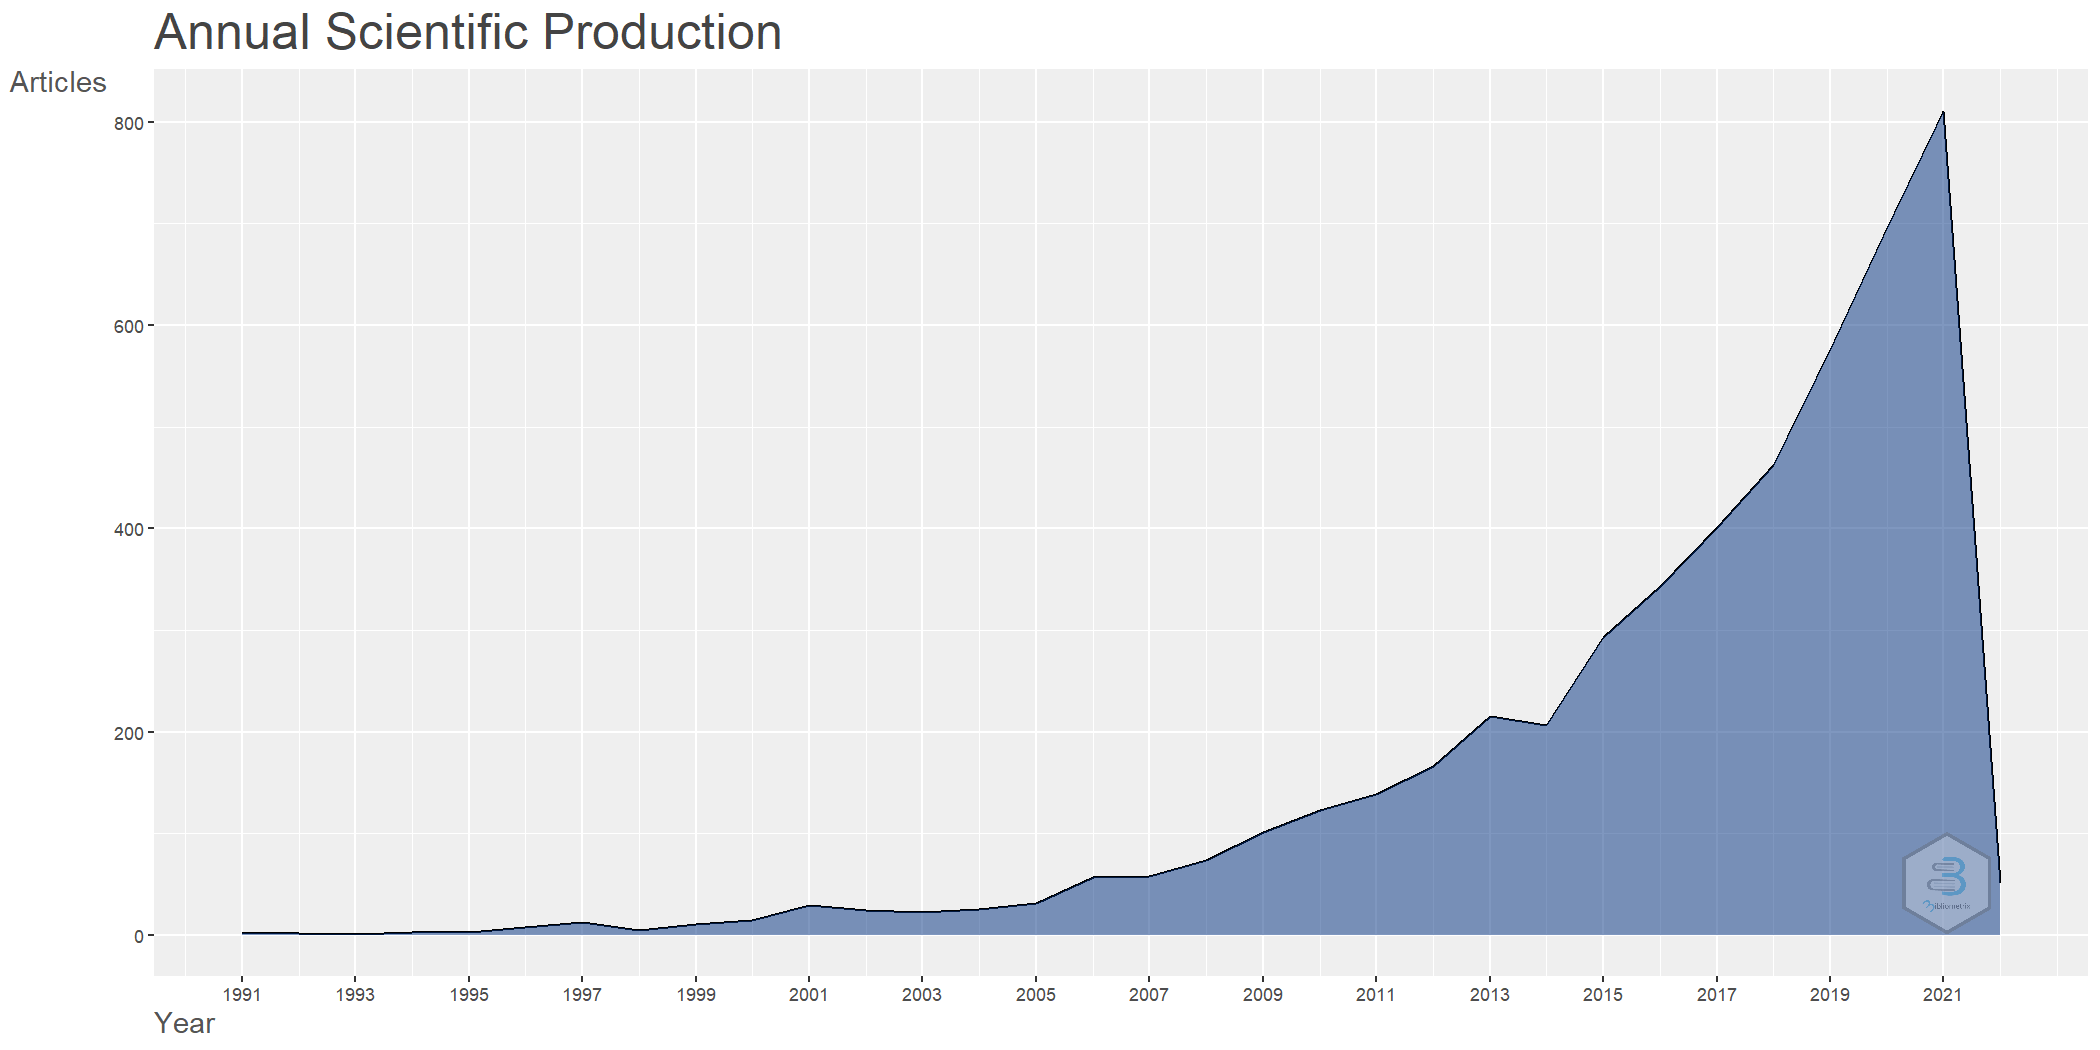
\includegraphics[width=1\textwidth]{experiments/vinis-caixe/PesqBibliogr/MineracaoDados/WoS-20220204/Dataset/AnnualScientificProduction-2022-02-06.png}
    \caption{Evolução da produção científica no \dataset\ .}
    \label{fig:evol:anual:vinis-caixe}
\end{figure}

O \textit{Annual Growth Rate} do \dataset\ é de 11,01\%, tendo 2021 como ano de maior produção de artigos científicos e 1993 o ano com menor produção.

\subsection{Interpretação do Crescimento}

A alta taxa de crescimento indica que existe interesse em utilizar mineração de dados na área de saúde. O fato dos anos 2020 e 2021 terem a maior produção de artigos científicos sugere que o surgimento do coronavírus causou um aumento na pesquisa.

\subsection{Evolução das Citações}

\begin{figure}
    \centering
    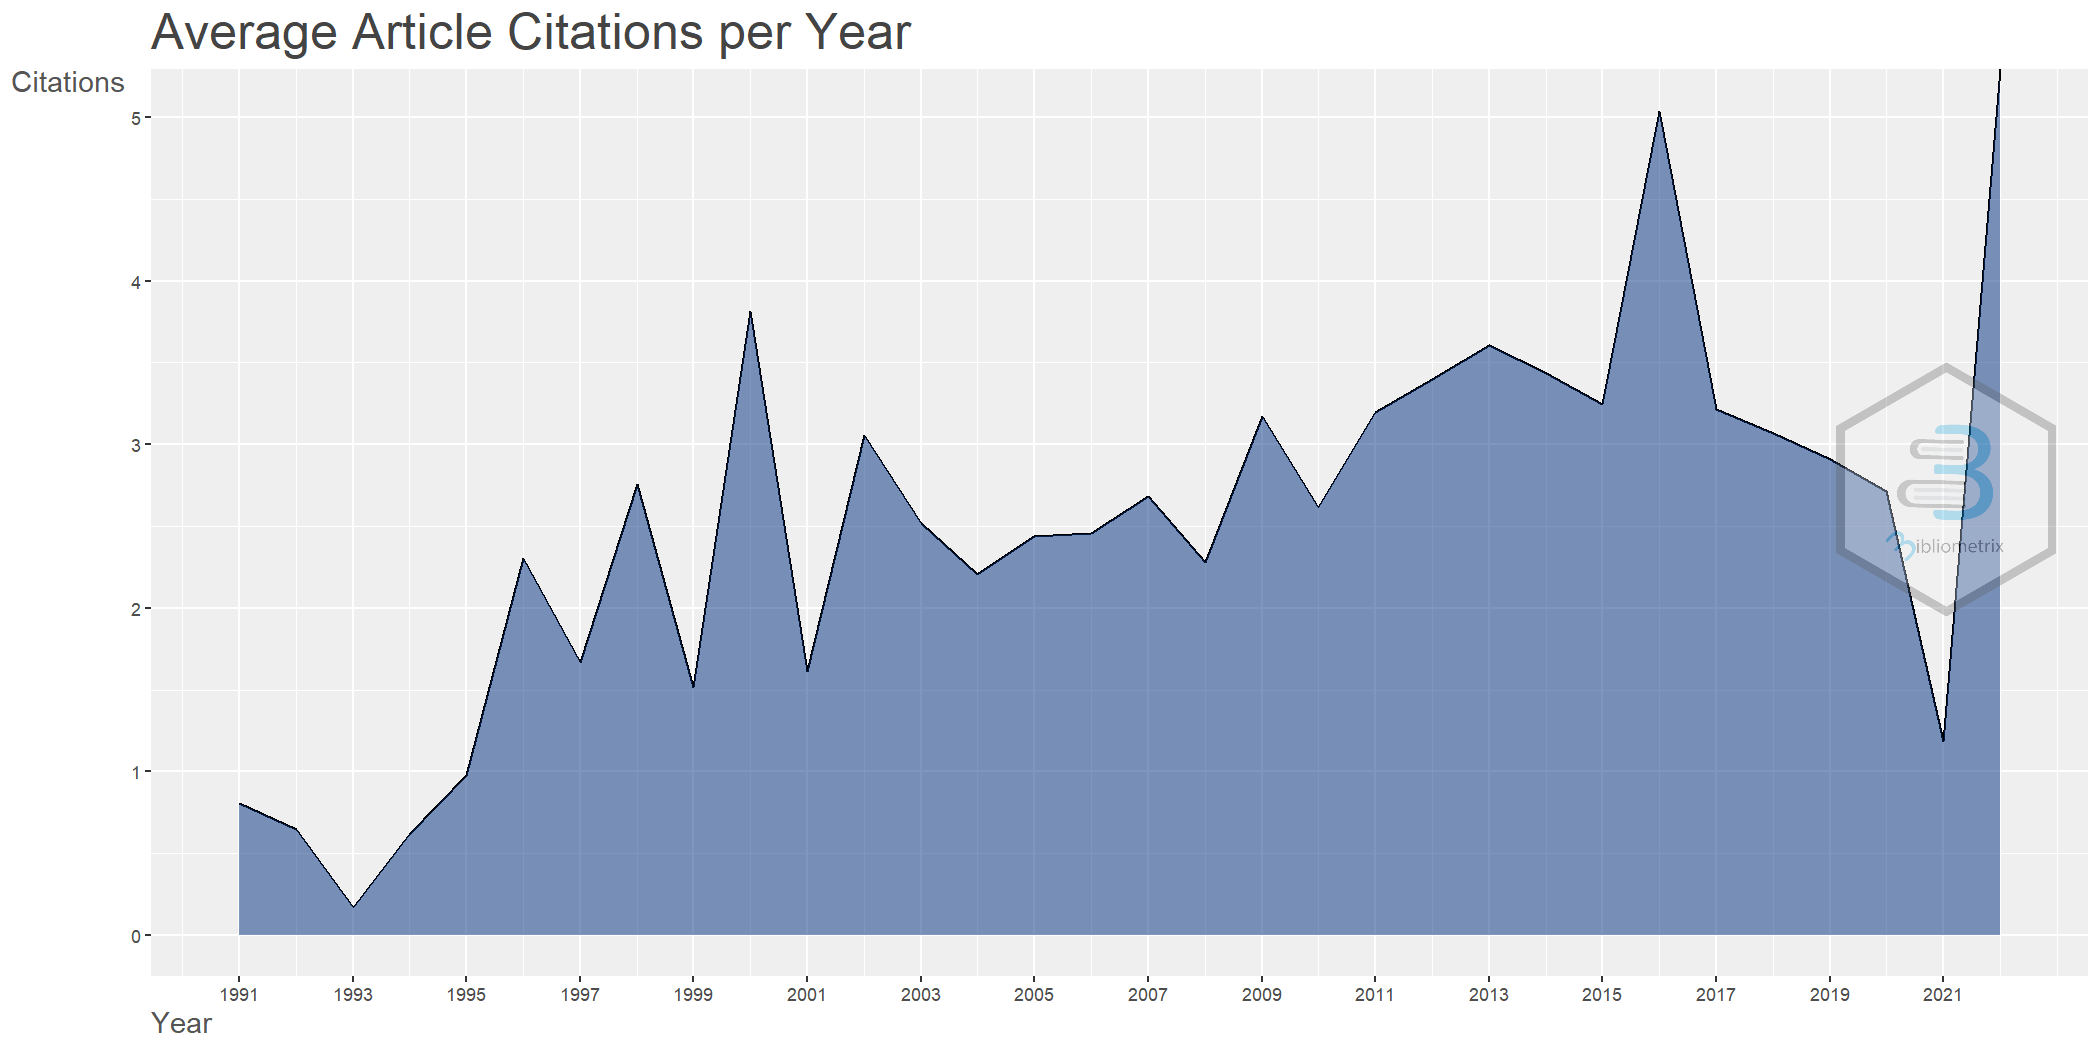
\includegraphics[width=1\textwidth]{experiments/vinis-caixe/PesqBibliogr/MineracaoDados/WoS-20220204/Dataset/AverageArticleCitationPerYear-2022-02-08.png}
    \caption{Média de citações por ano do \dataset\ .}
    \label{fig:cit:anual:vinis-caixe}
\end{figure}

\bibliographystyle{plainnat}
\bibliography{RESIC}

\end{document}.
